\chapter{Lifting holes to higher dimension}\label{ch:dimension}

A hole in $H_2$ lives on six ranks. If a seventh label is added, does the hole persist as a hole in $H_3$, and what in the arithmetic of the new label decides whether it does? This chapter develops a \emph{lift calculus} answering the first question at the level of chains and the second for the cases examined. The calculus is exact and elementary: it is the part of the programme where algebra rather than computation does most of the work, and every identity is proved in full. The arithmetic statements, which contents realise lifted holes, are finite or bounded and are labelled so.

\section{The lift operator}\label{sec:lift}
Faces of $P_k$ are ordered partitions of the rank set $\{0,\dots,k-1\}$ (\cref{def:faces}). Fix a new rank $n=k$ and regard $P_{k+1}$ as the permutohedron on $\{0,\dots,k\}$. All chains are over $\F$.
@@def:lift@@
@@RAW:ch08.tex::All three maps raise::of dimension $j{+}1$).@@

@@lem:LT0@@
@@thm:lift-cycle@@
@@RAW:ch08.tex::\begin{remark}[two fillings glued along $z$]::\end{remark}@@

\begin{figure}[ht]\centering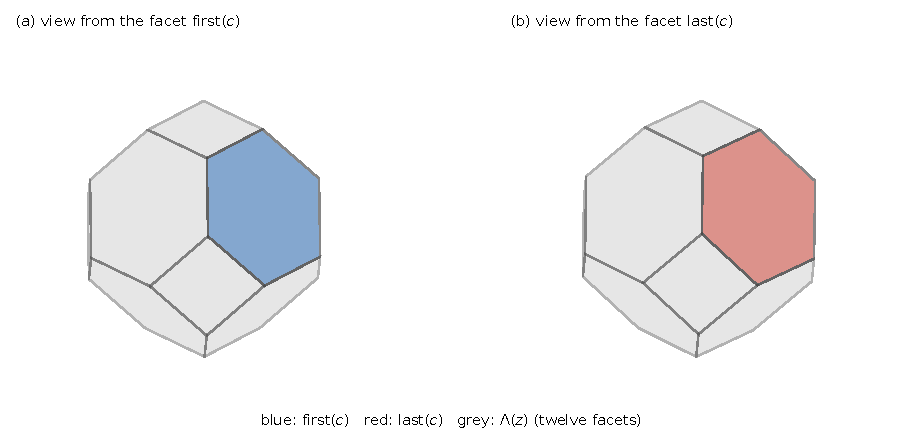
\includegraphics[width=\textwidth]{figures/fig_lift_diagonal.pdf}
\caption{The simplest lift, drawn from exact coordinates. Take the hexagon of $P_3$: its boundary $z$ is a $1$-cycle with the unique filling $c$, so the only lift is the diagonal one. Then $\Lambda(c)$ is the whole permutohedron $P_4$ (a truncated octahedron), $\first(c)$ and $\last(c)$ are the two hexagonal facets at which the new label $3$ is first or last (blue and red), and $\Lambda(z)$ is the band of the remaining twelve facets (grey). The identity $\partial\Lambda(c)=\Lambda(z)+\first(c)+\last(c)$ says that the three pieces together are the boundary sphere of $P_4$ (\cref{lem:LT0}). A non-diagonal lift needs two \emph{different} fillings of $z$.}\label{fig:lift}
\end{figure}

\section{The cochain lift}
@@thm:cochain-lift+computer-assisted obstruction set@@
@@cor:lifted-hole@@

\section{Certified examples and the arithmetic census}
@@prop:H3-examples+finite-exact@@
@@prop:lift-pairs+finite-exact@@
@@obs:nondeg+finite-exact@@
@@obs:AS1+bounded@@
Only the anchor class was censused for lifts. Whether every $H_3$ regime of a seven-label content is a lift is not known; the census covers only lifted patterns.

\section{Filling dependence}\label{sec:filldep}
The lift depends on two fillings. Is its homology class an invariant of $z$ alone, or does it remember how $z$ was filled? The answer is exact.
@@thm:filling-dependence@@
@@thm:FI-anchor+finite-exact@@
\emph{Does the topology of a generative history space depend only on which lower-dimensional cycles can be filled, or also on the relations between their alternative fillings?} By \cref{thm:filling-dependence,thm:FI-anchor} it depends also on the relations, and exactly through whether $\first(c_a+c_a')$ bounds in the complex.

\section{Iterated lifts and role maps}
@@thm:iterated-lift@@
@@obs:rolemap+finite-exact@@

\section{The filling-dependence map}\label{sec:JX}
@@def:JX@@
@@thm:JX@@
The lifted homology therefore depends on two things: \emph{which} cycles fill (the survival laws of \cref{thm:AT1}), and the lower-dimensional homology of the first-facet complex $F_X$, the freedom of filling relations being exactly the part of $H_j(F_X)$ that survives in $H_j(X)$.

\section{Scope of the lift results}
General-dimension statements are limited to the chain-level calculus: \cref{lem:LT0}, \cref{thm:lift-cycle}, \cref{thm:filling-dependence}, parts (J-1), (J-2) and (J-6) of \cref{thm:JX}, and part (HL-1) of \cref{thm:iterated-lift}. Everything that names a content is finite or bounded: non-degeneracy of the off-diagonal lifts is verified for $554$ pairs but not proved in general, injectivity of $\first_\ast$ is verified instance by instance, and the four-dimensional example is a certified single content with seven further verified neighbours. Figure~\ref{fig:lift} and the tables above are evidence about the anchor class and the identity role map at labels $\le30$, not a classification of $H_3$.
